% !TEX root = ../example_paper.tex

\section{Hardware}
\label{sec:hardware}
Kolesá a ozubené koliečko pre hriadeľ motora boli vytlačené v 3D tlačiarni s resinovou náplňou \textbf{FabPro 1000 Resin Cartridge Tough BLK}. Na obrázkoch \ref{fig:gear} a \ref{fig:wheel_w_gear} môžeme vidieť návrhy ozubeého koliečka pre hriadeľ a kolesa. 

\begin{figure}[!htbp]
        \centering
        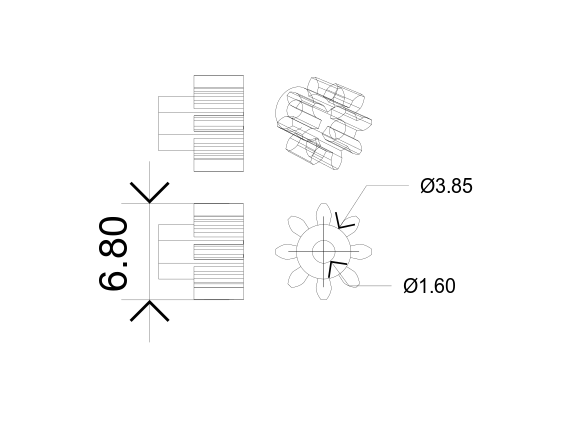
\includegraphics[scale=0.8]{includes/images/motor_gear.png}
        \caption{Užívateľské rozhranie s označenými komponentami}
        \label{fig:gear}
\end{figure}

\begin{figure}[!htbp]
        \centering
        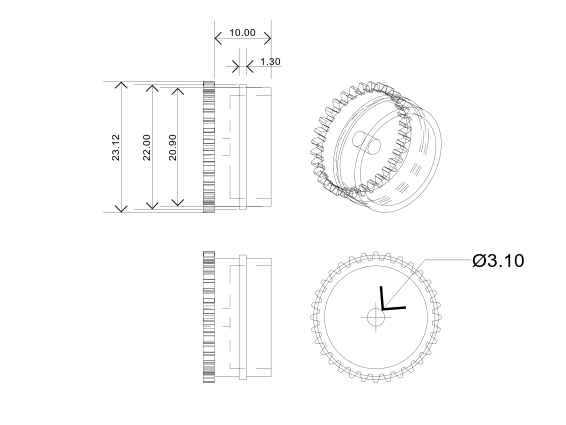
\includegraphics[scale=0.8]{includes/images/wheel_w_gear_2_blueprint.png}
        \caption{Koleso s ozubenými kolesami}
        \label{fig:wheel_w_gear}
\end{figure}

\section{Software}
\label{sec:software}

Na písanie kódu sme použili prostredie \textbf{esp\_idf} verzie \textit{4\.4\.7}, ktoré sme vytvorili za~pomoci
ich repozitára \cite{espGithub}.

Postup na~inicializáciu ESP IDF a~následné spustenie projektu je nasledovný:
\begin{enumerate}
	\item Stiahnutie ESP IDF z~repozitára \cite{espGithub} (My sme použili verziu 4.4.7).
	\item Spustenie príkazu \textit{./install.sh esp32} pre~Linux.
		Tento príkaz stiahne a~nainštaluje všetky potrebne závislosti.
	\item Exportovanie súboru \textit{. ./export.sh} pre~Linux.
		Tento príkaz nastaví všetky potrebne premenne prostredia.
	\item Zmeniť aktuálny adresár na~náš projekt.
	\item Spustiť príkaz \textit{idf.py build} pre~kompiláciu projektu.
	\item Spustiť príkaz \textit{idf.py -P <PORT\_NR> flash} pre~nahratie binárneho súboru do~ESP32.
		Pre tuto operáciu je potrebne mať pripojený počítač a~misku cez UART.
	\item Spustiť príkaz \textit{idf.py monitor} pre~sledovanie výstupu z~ESP32.
\end{enumerate}

Alternatívne spustenie je možné pomocou platformy \textbf{Visual Studio Code} s~nainštalovaným rozšírením
\textbf{ESP-IDF}~\cite{espIDF}.

\subsection{Odometria}
\label{subsec:odometria}

% Pridat referencia na~motor a~enkoder ked budu vytvorene v~hardweri
Podobne ako v~predmete \textit{Riadenie mobilných robotov} sme použili odometriu na~výpočet polohy robota.
Použili sme na~to inkrementálny enkóder, ktorý je pripojený na~motor. Z enkóderov si získame aktuálnu polohu robota
cez základný vzťah:

\begin{equation}
	\label{eq:odometria}
	 \Delta x_t = x_{t-1} + \Delta s_t \cdot \cos(\theta_{t-1} + \Delta \theta_t)
\end{equation}
\begin{align*}
	\Delta y_t = y_{t-1} + \Delta s_t \cdot \sin(\theta_{t-1} + \Delta \theta_t)
\end{align*}

\newpage

\subsection{PID}
\label{subsec:pid}

Do motorov posielame ako akčný zásah signál PWM (\acrlong{PWM}). Tento signál môže nadobúdať hodnoty od~0 po~1023.
Zároveň musíme myslieť aj na~prepäťovú ochranu. Keď pošleme do~motorov veľké zrýchlenie, tak sa stane, že sa program
na~čipe zresetuje.

Aby sme ošetrili tieto situácie, tak sme neimplementovali PID regulátor s~antiwindup zapojením. Jeho obmedzenie je
nastavené zdola na~0 a~zhora na~1023. Toto obmedzenie zdola je nastavené na~0 kvôli implementácii nastavenia smeru
otáčania motorov. V~prostredí ESP musíme dopredu nastaviť smer otáčania motorov. Po jeho nastavení sa všetky hodnoty
posielajú ako \textit{unsigned}. Teda ak by sme mu poslali zápornú hodnotu, tak by sa motor rozbehol nastaveným smerom.
Antiwindup zapojenie by maximálnu rýchlosť obmedzilo na~1023.

Pre jednoduchosť ovládania sme nastavili regulátor tak, aby vstupná žiadaná hodnota bol v~milimetroch za~sekundu.
Regulátor si túto hodnotu prepočíta na~PWM signál, ktorý pošle motorom. Spätné väzby sa získavajú z~enkóderov
a~dopočítavajú sa na~milimetre za~sekundu. Tieto hodnoty sa taktiež prepočítajú na~PWM signál. Prepočet z~milimetrov
za sekundu na~PWM signál je závislý uskutočňovaný nasledujúcim výpočtom:

\begin{equation}
	\text{PWM} = d \pi \frac{IMP_t}{IMP_{pr} i \Delta t}
	\label{eq:mmps2pwm}
\end{equation}

Rovnica \ref{eq:mmps2pwm} obsahuje parametre:
\begin{itemize}
	\item d - Priemer kolesa,
	\item $IMP_t$ - Aktuálne impulzy z~enkóderu,
	\item $IMP_{pr}$ - Impulzy z~enkóderu za~jednu otáčku (per rotation),
	\item i - Pomer prevodovky motora. Na~našich motoroch je to prevod 32:8,
	\item $\Delta t$ - Časový interval od~posledného merania
\end{itemize}

